%   % !TEX root = ../../VIII,3_Rahmen-TeX_8-1.tex
%  
%   Band VIII, 3		Rubrik STOSS
%
%   Signatur/Tex-Datei:	35_10_07_009-010
%				
%   RK-Nr. 	60038		
%
%   N.~\ref{RK60038}
%
%   Überschrift: 	(keine)
%   
%   Unterrubrik:			Überblick
%
%   edlabels:			1		(wieviele?)
%
%   Diagramme: 		9
%
%
%   NB: 						(Anmerkungen)					??
%
%
%
\selectlanguage{ngerman}
\frenchspacing
%
\begin{ledgroupsized}[r]{120mm}
\footnotesize
\pstart
\noindent\textbf{Überlieferung:}
\pend
\end{ledgroupsized}
%
\begin{ledgroupsized}[r]{114mm}
\footnotesize
\pstart \parindent -6mm
\makebox[6mm][l]{\textit{L}}%
Aufzeichnung:
LH~XXXV~10, 7 Bl.~9\textendash10. 
Ein Bogen~4\textsuperscript{o};
Gegenmarke eines Wasserzeichens im Falz (Wiener Papier).
Zweieindreiviertel Seiten auf Bl.~9~r\textsuperscript{o} bis Bl.~10~r\textsuperscript{o}; Bl.~10~v\textsuperscript{o} ist unbeschrieben.
\pend
\end{ledgroupsized}
%
%
\vspace{5mm}
\begin{ledgroup}
\footnotesize
\pstart
\noindent%
\textbf{Datierungsgründe:}
Die vorliegende titellose Aufzeichnung N.~\ref{RK60038} ist auf Papier verfasst, das sich anhand des Wasserzeichens auf Leibnizens ersten Aufenthalt in Wien (Mai 1688 bis Februar 1689) datieren lässt.
Die Entstehungszeit lässt sich jedoch weiter einschränken.
Die Verwendung der Begriffe \textit{vis insita} (S.~\refpassage{LH_35_10_07_009r_visinsita-1}{LH_35_10_07_009r_visinsita-2}) und \textit{quantitas centripeta vel centrifuga} (S.~\refpassage{LH_35_10_07_0010r_centripetafuga-1}{LH_35_10_07_0010r_centripetafuga-2}) sowie die grundlegende Fragestellung, die die Auseinandersetzung mit der Stoßlehre in N.~\ref{RK60038} offenbar veranlasst \textendash\ nämlich eine rein mechanistische Erklärung der Wurf- und Umlaufbahn (vgl. S.~\refpassage{LH_35_10_07_009r_motivation-1}{LH_35_10_07_009r_motivation-2}) \textendash, setzen eine unmittelbare Auseinandersetzung mit
\protect\index{Namensregister}{\textso{Newton} (Neutonus), Isaac 1643\textendash1727}%
Newtons \textit{Principia} (1687)\cite{00535} voraus,
oder wenigstens eine Lektüre der von C.~Pfautz%
\protect\index{Namensregister}{\textso{Pfautz} (Pfauzius), Christoph 1645\textendash1711}
veröffentlichten, ausführlichen Besprechung von Newtons Abhandlung (\textit{AE}, Juni 1688, S.~303\textendash315).\cite{01356}
Mit den \textit{Principia} \textendash\ insbesondere dem ersten Lehrsatz (lib.~I, sect.~II, prop.~1, S.~37\,f.)\cite{00535} \textendash\ befasst sich ebenfalls der im Herbst 1688 niedergeschriebene Entwurf \textit{Physico-mechanicae leges} (N.~\ref{RK60323} in diesem Band; siehe für die Einzelheiten die Datierungsgründe auf S.~\pageref{LH_37_05_104-105_datierung}).
Am Ende dieses Textes skizziert Leibniz gleichsam das Programm für die Fortsetzung der Untersuchung (S.~\refpassage{LH_37_05_105v_Vorverweis-1}{LH_37_05_105v_Vorverweis-2}):
Es gelte insbesondere zu prüfen, ob das Prinzip der \textit{compositio motuum} \textendash\ und somit die \glqq Schiff\grqq-Methode \textendash\ auch auf Fälle schiefen und mehrfachen Stoßes anwendbar bleibe.
Zu diesem Zweck sei es methodisch von der \glqq fiktionalen\grqq\ Annahme auszugehen, dass die zusammenstoßenden Körper sich nach Belieben als zusammenhängend oder abgetrennt auffassen ließen.
\edlabel{LH_35_10_07_009-010_Datierung-1}%
An dieses in N.~\ref{RK60323} skizzierte \glqq Arbeitsprogramm\grqq\ knüpft offenbar die Aufzeichnung N.~\ref{RK60038} an:
Hier werden in systematischer Ordnung Fälle mehrfachen Stoßes untersucht, und zwar unter den methodischen Annahmen, die am Ende von N.~\ref{RK60323} kurz dargelegt werden.%
\edlabel{LH_35_10_07_009-010_Datierung-2}
Der Zusammenhang beider Texte wird auch bei den Zeichnungen sichtbar:
Das Diagramm \lbrack\textit{Fig.~5}\rbrack\ in N.~\ref{RK60323} (S.~\pageref{LH_37_05_105v_Fig.5}), das keine Verbindung mit dem dortigen Text aufweist, zeigt indessen auffällige Ähnlichkeit mit dem Diagramm \lbrack\textit{Fig.~2}\rbrack\ in N.~\ref{RK60038} (S.~\pageref{LH_35_10_07_009r_Fig.2}).
Aus dieser inhaltlichen Abhängigkeit folgt, dass N.~\ref{RK60038} nicht vor N.~\ref{RK60323}, d.h. nicht vor dem Herbst 1688, entstanden sein kann, aller Wahrscheinlichkeit nach aber noch vor Leibnizens Abfahrt aus Wien in Februar 1689 angefertigt wurde.
Hieraus ergibt sich die vorgeschlagene Datierung.
%
\pend%
\end{ledgroup}%
%
%
\selectlanguage{latin}%
\frenchspacing%
\newpage%
% \vspace{8mm}%
\pstart%
\normalsize%
\noindent%
%
\lbrack9~r\textsuperscript{o}\rbrack\    % % % %    Blatt 9r
%
%
Si corpus \textit{LM} incurrat%
\protect\index{Sachverzeichnis}{corpus incurrens}
in corpus \textit{AB},
demonstratum est 
%
\edtext{alibi}{%
\lemma{alibi}\Cfootnote{%
Vermutlich Anspielung auf den ersten Teil von N.~\ref{RK60323}, wo Leibniz in Anlehnung an N.~\ref{RK41201} die Gesetze des direkten zentralen Stoßes unter den angegebenen Annahmen nachweist.
Den Erhalt der \textit{potentia} (d.h. der Kraft $mv^2$) und der \textit{directio} (d.h. der gleichförmigen Bewegung des gemeinsamen Schwerpunkts) hat Leibniz wiederum in % den \textit{schedae} VIII bzw. IX 
\textit{De corporum concursu} (N.~\ref{dcc_08} und N.~\ref{dcc_09}) nachgewiesen.%
}}
%
\edtext{ex lege conservandae}{%
\lemma{ex}\Bfootnote{%
\textit{(1)}~natura ser
\textit{(2)}~lege conservandae%
~\textit{L}}}
%
potentiae%
\protect\index{Sachverzeichnis}{lex conservandae potentiae}%
\protect\index{Sachverzeichnis}{potentia conservanda}
et directionis,%
\protect\index{Sachverzeichnis}{lex conservandae directionis}%
\protect\index{Sachverzeichnis}{directio conservanda}
quid sit futurum. \pend 
%
%
\vspace{1.0em} %%%%%%%%% Diagramm 1
\centerline{%
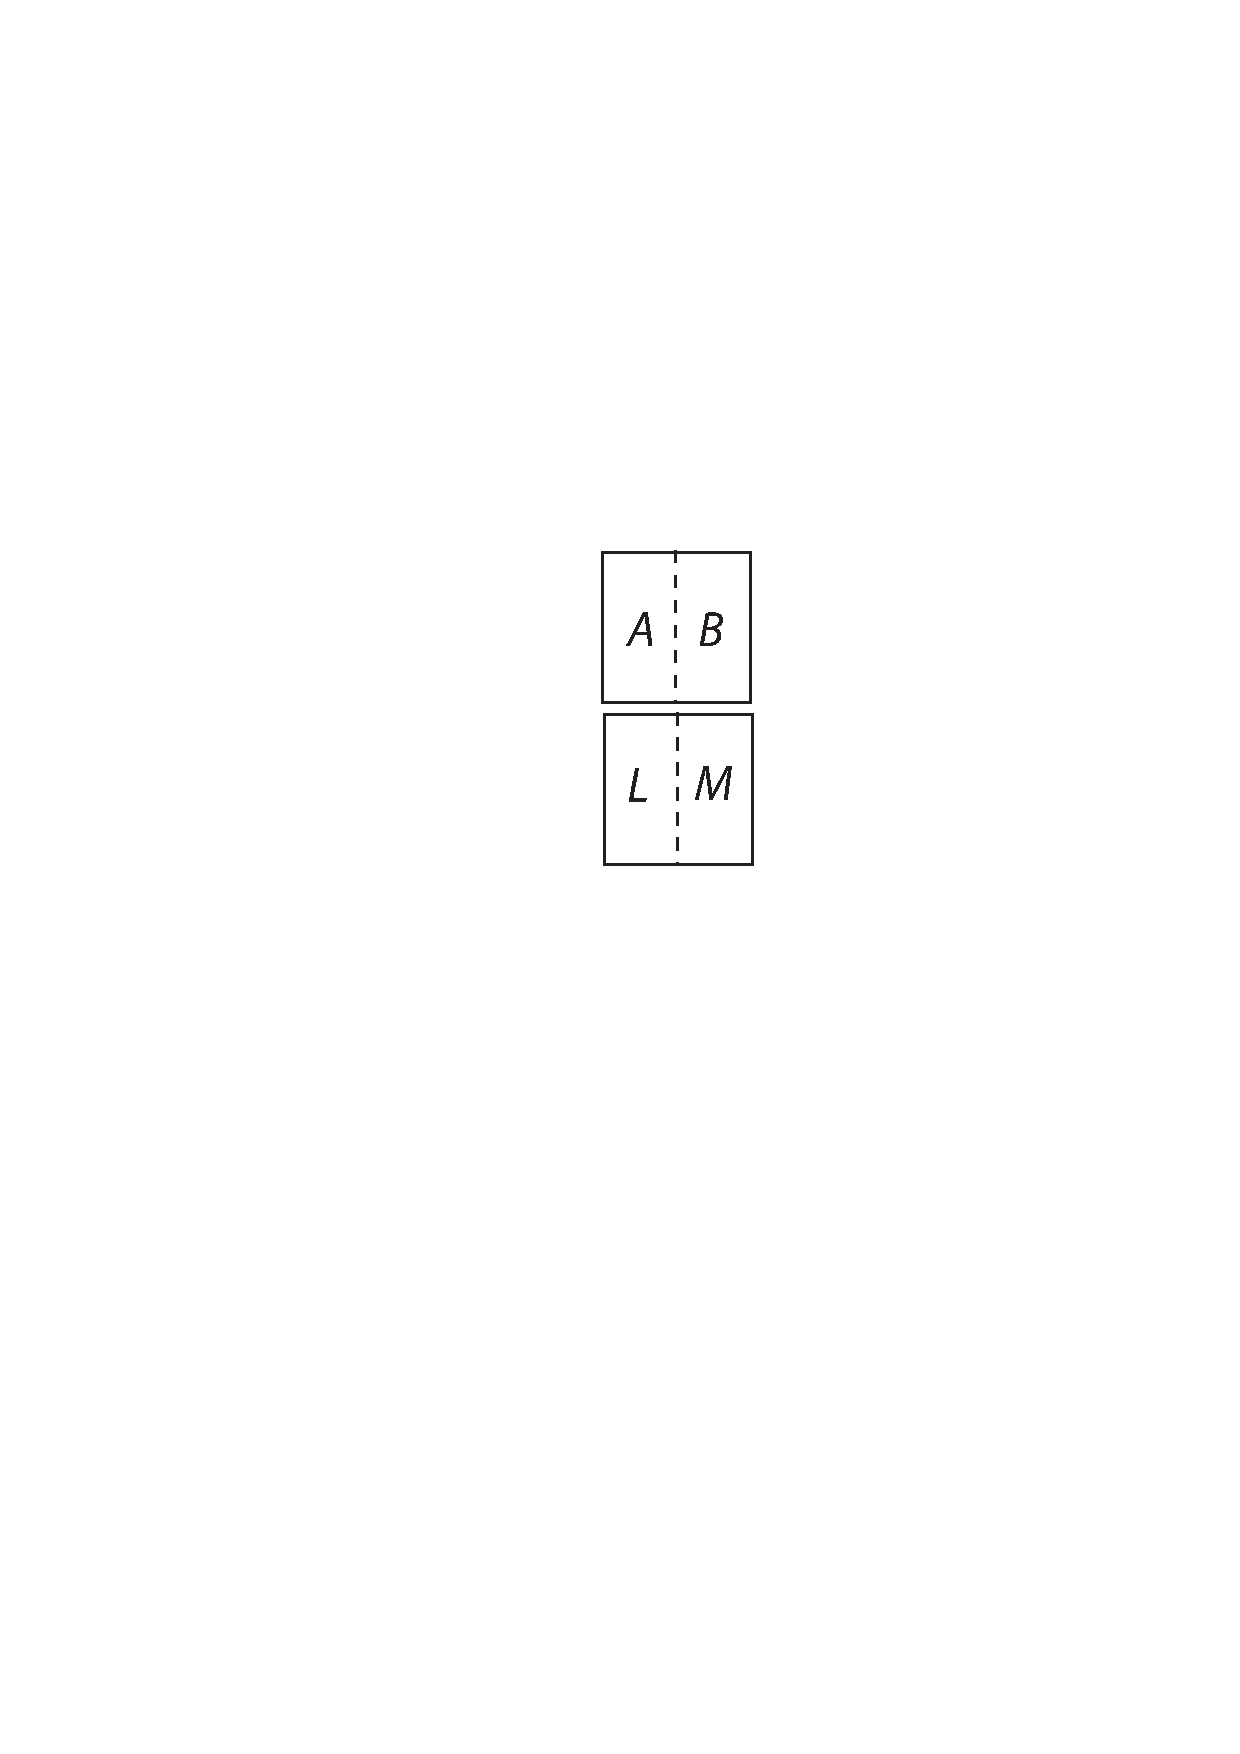
\includegraphics[width=0.09\textwidth]{%
gesamttex/edit_VIII,3/images/LH_35_10_07_009-010_d1_009r.pdf%
}}
\vspace{0.5em}
\centerline{%
\lbrack\textit{Fig.~1}\rbrack%
}
% \newpage%
\vspace{1.0em}
%
\pstart%
Sed si 
%
\edtext{ponamus corpora%
\protect\index{Sachverzeichnis}{corpora duplicia}
\textit{AB} et \textit{LM} duplicia,
et \textit{AB} simile equidem esse
et similiter positum ipsi \textit{LM},
neutrum tamen%
}{%
\lemma{ponamus}\Bfootnote{%
\textit{(1)}~corpus
\textit{(2)}~corpora \textit{AB} et \textit{LM}
\textbar~et \textit{streicht Hrsg.}~%
\textbar\ duplicia, et \textit{AB}
\textit{(a)}~similiter
\textit{(b)}~simile equidem % esse et similiter positum 
\lbrack...\rbrack\ ipsi \textit{LM},
\textit{(aa)}~sed
\textit{(bb)}~neutrum tamen%
~\textit{L}}}
%
esse cohaerens%
\protect\index{Sachverzeichnis}{corpus cohaerens}
atque unum,%
\protect\index{Sachverzeichnis}{corpus unum}
sed ambo constare,
illud ex \textit{A} et \textit{B},
hoc ex \textit{L} et \textit{M},
quae iterum similia et similiter posita,%
\protect\index{Sachverzeichnis}{corpora similia et similiter posita}
tunc utique omnia orientur %,
quae ante,
perinde ac si ambo corpora essent firma,%
\protect\index{Sachverzeichnis}{corpus firmum}
seu perinde ac si \textit{A} et \textit{B}
unum corpus firmum componerent,
ac similiter \textit{L} et \textit{M},
ut facile demonstrari potest.
\pend%
%
%
\vspace{1.0em} %%%%%%%%% Diagramm 2
\centerline{%
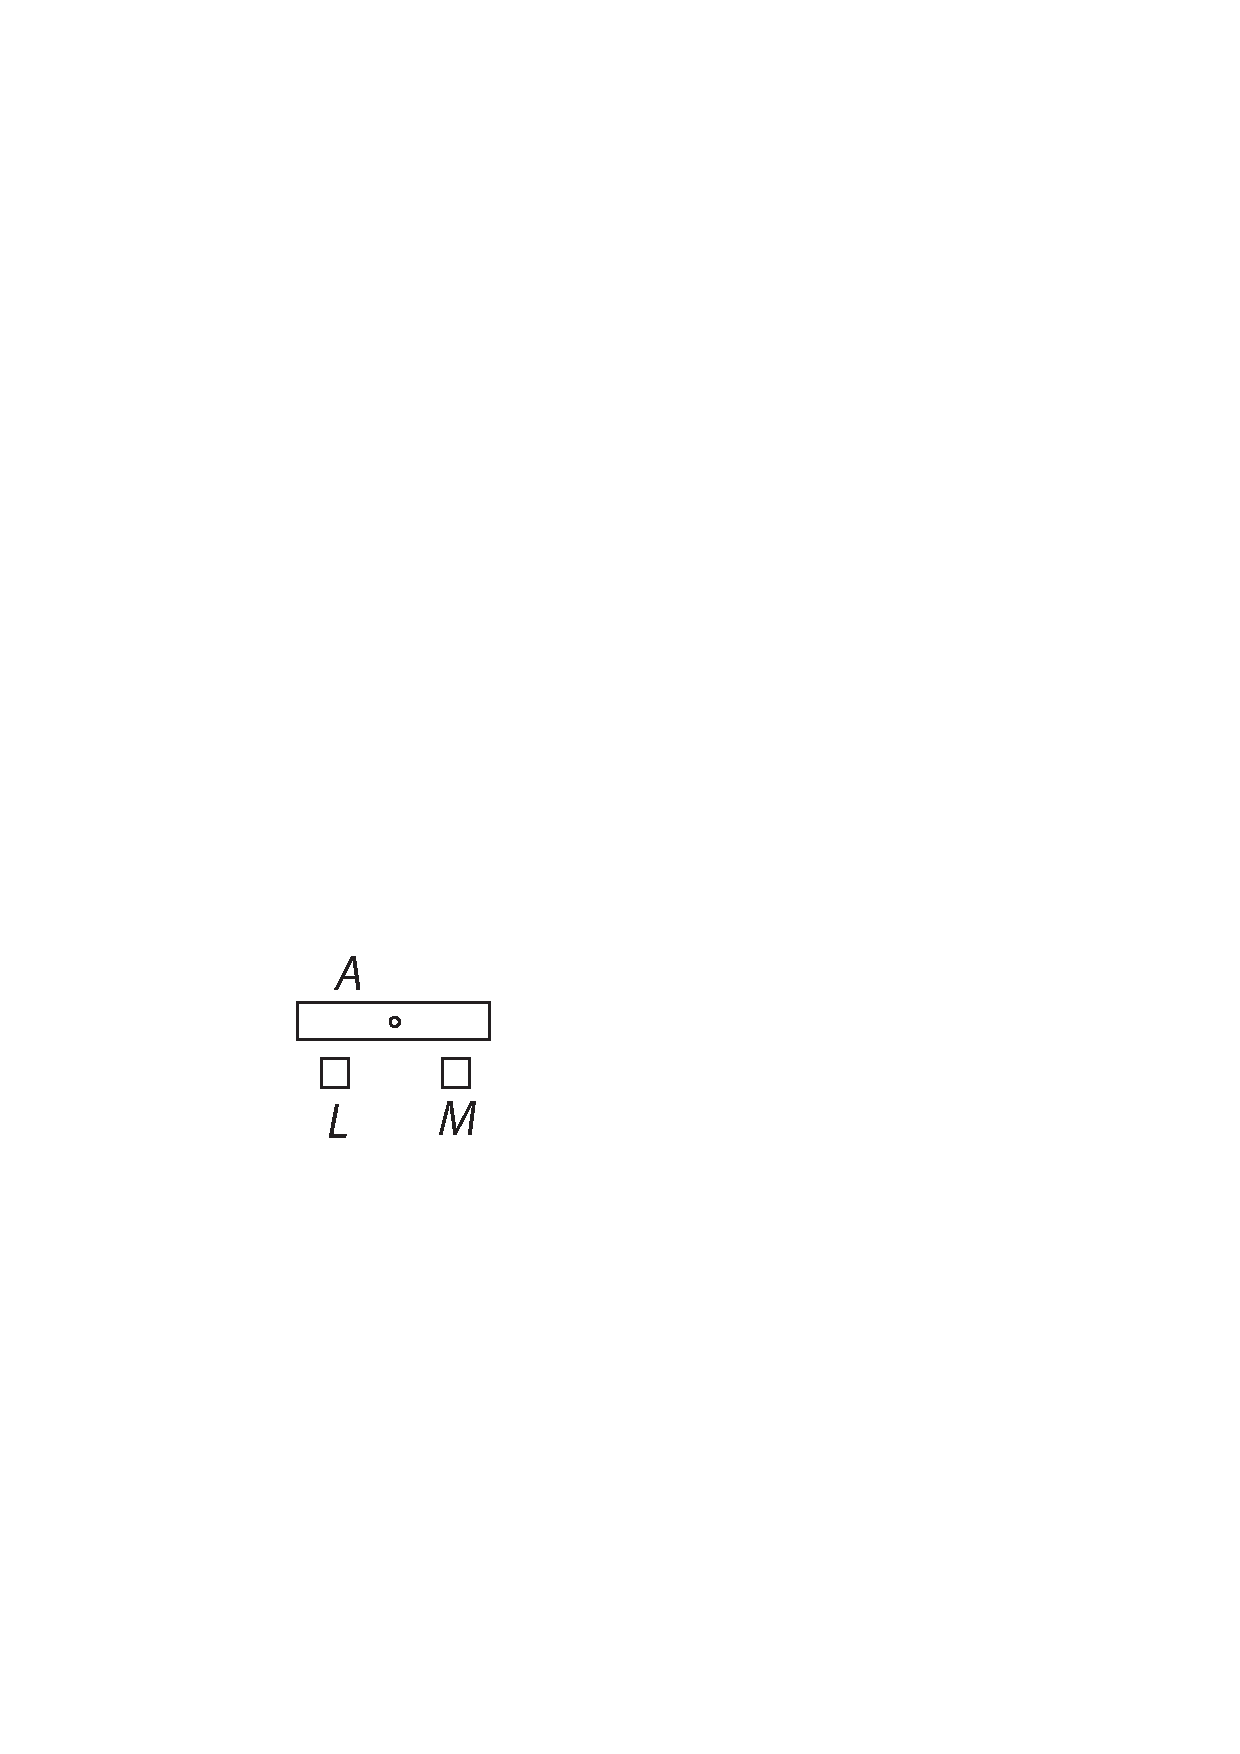
\includegraphics[width=0.11\textwidth]{%
gesamttex/edit_VIII,3/images/LH_35_10_07_009-010_d2_009r.pdf%
}}
\vspace{0.5em}
\centerline{%
\lbrack\textit{Fig.~2}\rbrack%
\label{LH_35_10_07_009r_Fig.2}%
}
% \newpage%
\vspace{1.0em}
%
\pstart%
Sed quod si ponamus
alterutrum esse firmum,%
\protect\index{Sachverzeichnis}{corpus firmum}
alterum esse solutum,%
\protect\index{Sachverzeichnis}{corpus solutum}
nihilominus dicendum erit
idem oriri,
cum ambobus et solutis
eodem modo resilientibus,%
\protect\index{Sachverzeichnis}{corpus resiliens}
perinde sit,
ac si idem adhuc sit corpus,
neque enim ob ictum%
\protect\index{Sachverzeichnis}{ictus}
a se invicem separantur licet soluta.%
\protect\index{Sachverzeichnis}{corpus solutum}
Itaque generaliter,
si duo corpora
%
\edtext{\textit{L,\:M}}{%
\lemma{\textit{L,\:M}}\Bfootnote{%
\textit{erg.~L}}}
%
impingant in tertium \textit{A},%
\protect\index{Sachverzeichnis}{corpora impingentia in tertium}
atque ita quidem ut nulla sit causa%
\protect\index{Sachverzeichnis}{causa}
cur non post ictum%
\protect\index{Sachverzeichnis}{ictus}
eandem quam antea distantiam servent,%
\protect\index{Sachverzeichnis}{distantia corporum ante ictum}%
\protect\index{Sachverzeichnis}{distantia corporum post ictum}
eadem orientur phaenomena,%
\protect\index{Sachverzeichnis}{phaenomenon}
ac si duo corpora fuissent firmiter connexa,%
\protect\index{Sachverzeichnis}{corpus connexum}
seu constituissent corpus unum.%
\protect\index{Sachverzeichnis}{corpus unum}
\pend%
\newpage
%
%
\vspace{1.0em} %%%%%%%%% Diagramm 3
\centerline{%
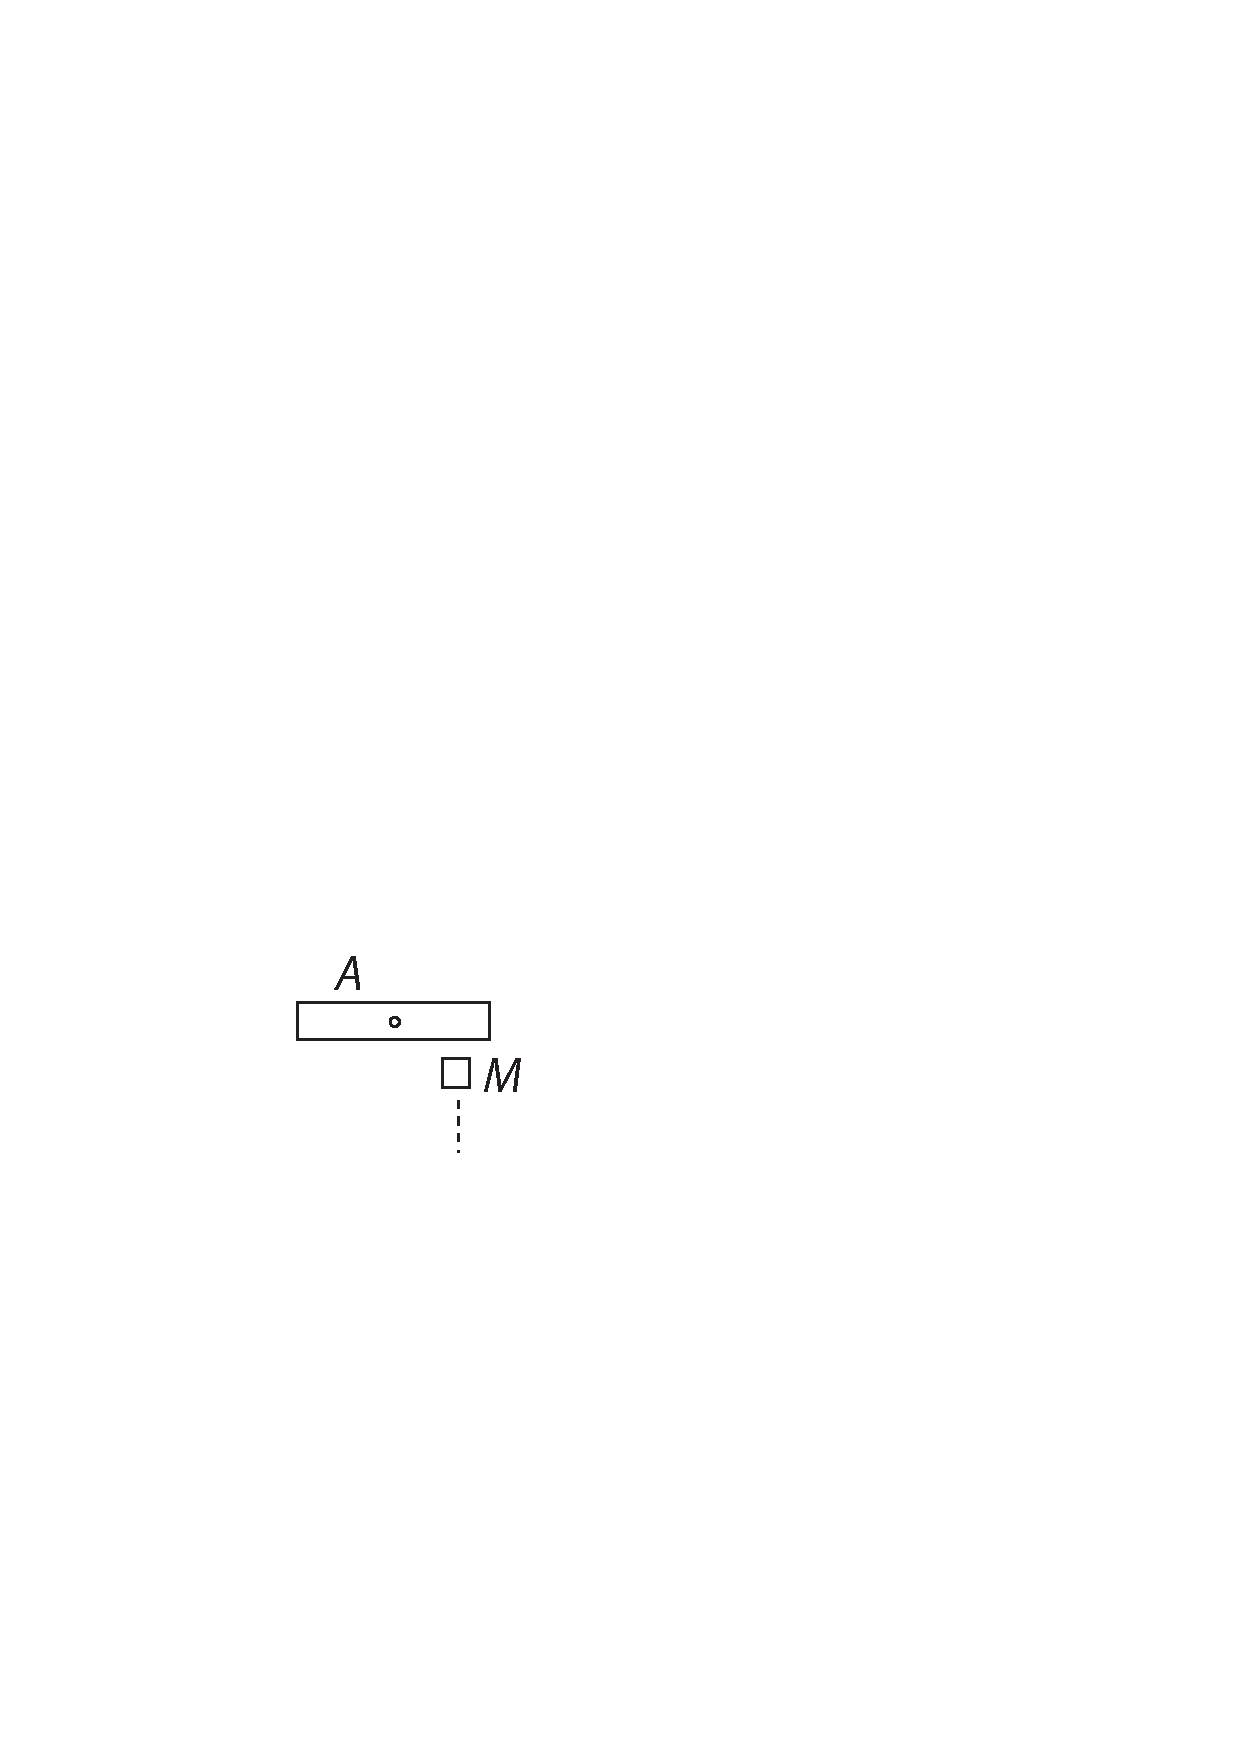
\includegraphics[width=0.13\textwidth]{%
gesamttex/edit_VIII,3/images/LH_35_10_07_009-010_d3_009r.pdf%
}}
\vspace{0.3em}
\centerline{%
\lbrack\textit{Fig.~3}\rbrack%
}
% \newpage%
\vspace{1.0em}
%
%
\pstart%
Si in corpus \textit{A} impingat corpus \textit{M}%
\protect\index{Sachverzeichnis}{corpus impingens}%
\protect\index{Sachverzeichnis}{corpus impactum}%
\protect\index{Sachverzeichnis}{impactus non directus}%
\protect\index{Sachverzeichnis}{impactus obliquus}
linea non directa in centrum gravitatis%
\protect\index{Sachverzeichnis}{centrum gravitatis}
ipsius \textit{A} ita,
ut intelligi possit
%
\edtext{corpus \textit{A} non tantum%
\protect\index{Sachverzeichnis}{corpus propulsum ab ictu}
directe propelli ab hoc ictu,%
\protect\index{Sachverzeichnis}{ictus}
sed et gyrari,%
\protect\index{Sachverzeichnis}{corpus gyrans}%
}{%
\lemma{corpus \textit{A}}\Bfootnote{%
\textit{(1)}~simul gyrari
\textit{(2)}~non tantum % directe propelli ab hoc ictu, sed 
\lbrack...\rbrack\ et gyrari,%
~\textit{L}}}
%
definiendum est,
quae sit gyratio;%
\protect\index{Sachverzeichnis}{gyratio}
quae propulsio.%
\protect\index{Sachverzeichnis}{propulsio}
Videtur talis ineunda ratio,
ut omnia quam minime mutentur.%
\pend%
%
\vspace{1.0em} %%%%%%%%% Diagramm 4
\centerline{%
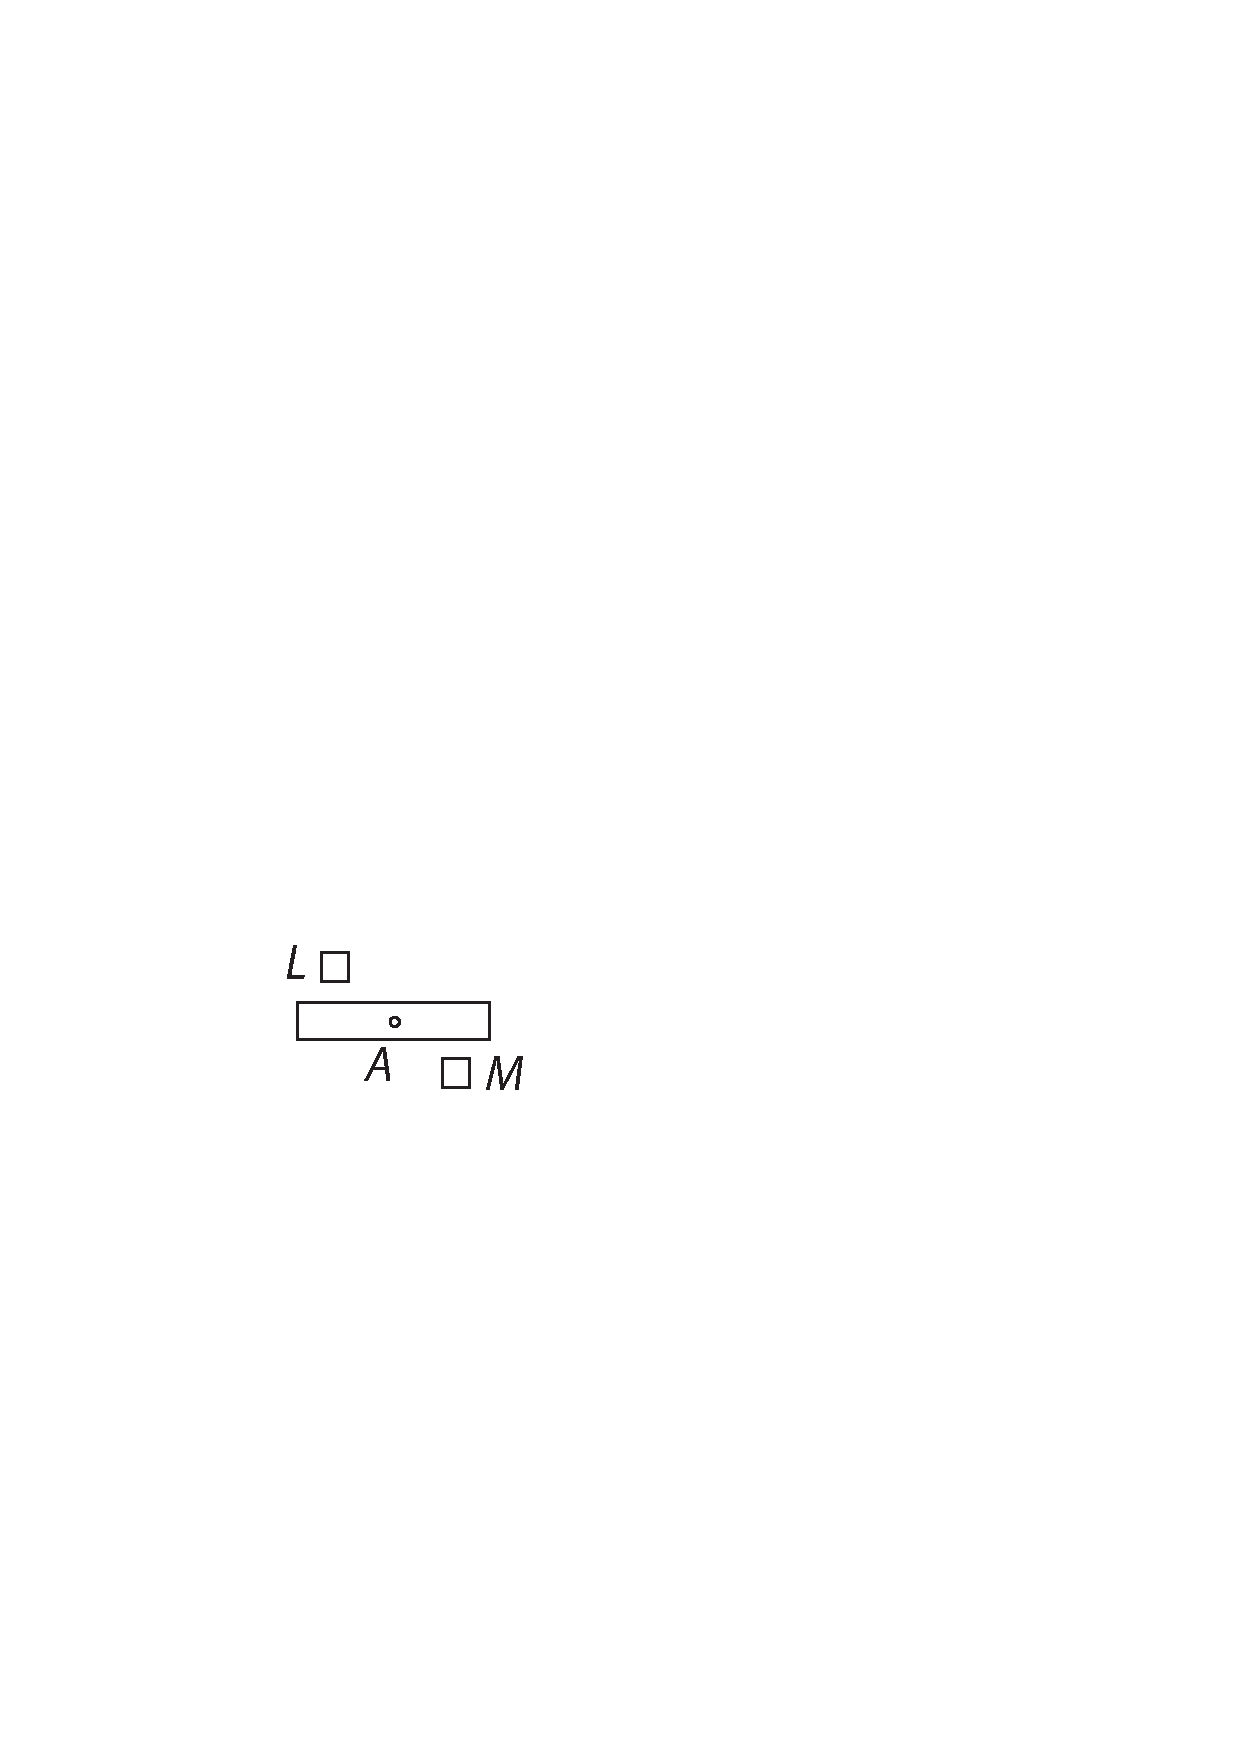
\includegraphics[width=0.13\textwidth]{%
gesamttex/edit_VIII,3/images/LH_35_10_07_009-010_d4_009r.pdf%
}}
\vspace{0.5em}
\centerline{%
\lbrack\textit{Fig.~4}\rbrack%
}
% \newpage%
\vspace{1.0em}
%
\pstart%
Si 
%
\edtext{in}{%
\lemma{in}\Bfootnote{%
\textit{erg.~L}}}
%
corpus \textit{A} impingant duo corpora%
\protect\index{Sachverzeichnis}{corpus impingens}
\textit{L} et \textit{M},
conspirantia ad eandem gyrationem%
\protect\index{Sachverzeichnis}{corpora conspirantia ad eandem gyrationem}%
\protect\index{Sachverzeichnis}{gyratio}
%
\edtext{ipsius \textit{A},}{%
\lemma{ipsius \textit{A}}\Bfootnote{%
\textit{erg.~L}}}
%
videndum est
quae lex gyrationis%
\protect\index{Sachverzeichnis}{lex gyrationis}%
\protect\index{Sachverzeichnis}{gyratio}
prodire debeat% ,
\lbrack;\rbrack\
corpus autem semel gyrans,%
\protect\index{Sachverzeichnis}{corpus gyrans}
si partes habeat satis firmas%
\protect\index{Sachverzeichnis}{pars corporis firma}
semper gyrabit.%
%\edtext{}{%
%\lemma{\hspace{1,6mm}\lbrack\textit{Fig.~5}\rbrack}\killnumber\Cfootnote{Die durch {\scriptsize \textit{3}}\textit{C} führende Gerade {\scriptsize \textit{3}}\textit{L}{\scriptsize \textit{3}}\textit{M} ist von Leibniz nicht eingezeichnet.}}
\pend%
%
\vspace{1.0em} %%%%%%%%% Diagramm 5
\centerline{%
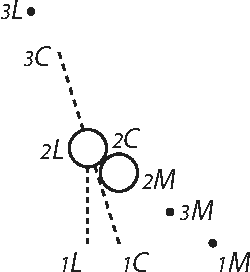
\includegraphics[width=0.22\textwidth]{%
gesamttex/edit_VIII,3/images/LH_35_10_07_009-010_d5_009r.pdf%
}}
\vspace{0.5em}
\centerline{%
\lbrack\textit{Fig.~5}\rbrack%
\label{LH_35_10_07_009r_Fig.5}%
}
% \newpage%
\vspace{1.0em}
%
\pstart 
Si in corpus \textit{L}%
\protect\index{Sachverzeichnis}{corpus impactum}
veniens celeritate%
\protect\index{Sachverzeichnis}{celeritas corporis impacti}
\textit{{\scriptsize \textit{1}}L{\scriptsize \textit{2}}L}
impingat corpus \textit{M}%
\protect\index{Sachverzeichnis}{corpus impingens}
celeritate%
\protect\index{Sachverzeichnis}{celeritas corporis impingentis}
\textit{{\scriptsize \textit{1}}M{\scriptsize \textit{2}}M},
quaeritur quid sit
%
\edtext{futurum.
Pro certo habendum est%
}{%
\lemma{futurum.}\Bfootnote{%
\textit{(1)}~Ponamus corpora esse
\textit{(a)}~puncta ut
\textit{(b)}~incomparabilis parvitatis seu ut puncta,
\textit{(2)}~Pro certo habendum est%
~\textit{L}}}
%
corpus \textit{M} manere in linea
\textit{{\scriptsize \textit{1}}M{\scriptsize \textit{2}}M},
si scilicet in
%
\edtext{momento incursus%
\protect\index{Sachverzeichnis}{incursus}%
\protect\index{Sachverzeichnis}{momentum incursus}%
}{%
\lemma{momento}\Bfootnote{%
\textit{(1)}~dire
\textit{(2)}~incursus\protect\index{Sachverzeichnis}{incursus}%
~\textit{L}}}
%
illa linea recta
per centrum ipsius
{\scriptsize \textit{2}}\textit{L}
transit.
Pro certo etiam haben- \makebox[1.0\textwidth][s]{dum est
viam centri gravitatis%
\protect\index{Sachverzeichnis}{centrum gravitatis commune}%
\protect\index{Sachverzeichnis}{via centri gravitatis}
%
\edtext{communis}{%
\lemma{communis}\Bfootnote{%
\textit{erg.~L}}}
%
manere eandem
\textit{{\scriptsize \textit{1}}C{\scriptsize \textit{2}}C},
ante et post concursum% ,
\protect\index{Sachverzeichnis}{concursus corporum}%
\lbrack;\rbrack}
\pend
\newpage
\pstart
\noindent
datur ergo
\textit{{\scriptsize \textit{2}}C{\scriptsize \textit{3}}C},
adeoque et punctum
{\scriptsize \textit{3}}\textit{C}.
Quod si ergo daretur et punctum
{\scriptsize \textit{3}}\textit{M} % ,
seu recta
\textit{{\scriptsize \textit{2}}M{\scriptsize \textit{3}}M},
necessario daretur et punctum
{\scriptsize \textit{3}}\textit{L},
quia
%
\edtext{recta \textit{{\scriptsize \textit{3}}L{\scriptsize \textit{3}}M}%
}{%
\lemma{recta \textit{{\scriptsize \textit{3}}L{\scriptsize \textit{3}}M}}\Cfootnote{%
Die durch {\scriptsize \textit{3}}\textit{C} führende
Gerade {\scriptsize \textit{3}}\textit{L}{\scriptsize \textit{3}}\textit{M}
ist im Diagramm \lbrack\textit{Fig.~5}\rbrack\
auf S.~\pageref{LH_35_10_07_009r_Fig.5} nicht eingezeichnet.%
}}
%
a puncto
{\scriptsize \textit{3}}\textit{C}
in data ratione secatur,
et
%
\edtext{\lbrack\textit{{\scriptsize \textit{3}}L{\scriptsize \textit{3}}C}\rbrack}{%
\lemma{\textit{{\scriptsize \textit{3}}M{\scriptsize \textit{3}}C}}\Bfootnote{%
\textit{L~ändert Hrsg.}}}
%
datur.
\pend%
%
\vspace{1.0em} %%%%%%%%% Diagramm 6
\centerline{%
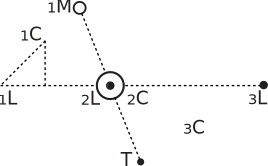
\includegraphics[width=0.40\textwidth]{%
gesamttex/edit_VIII,3/images/LH_35_10_07_009-010_d6_009r.pdf%
}}
\vspace{0.5em}
\centerline{%
\lbrack\textit{Fig.~6}\rbrack%
\label{LH_35_10_07_009r_Fig.6}%
}
% \newpage%
\vspace{1.0em}
%
\pstart%
%\edtext{}{%
%\lemma{\hspace{1,6mm}\lbrack\textit{Fig.~6}\rbrack}\killnumber\Cfootnote{%
%Die durch {\scriptsize \textit{1}}\textit{C}{\scriptsize \textit{2}}\textit{C}{\scriptsize \textit{3}}\textit{C} führende Gerade sowie die Punkte {\scriptsize \textit{2}}\textit{M} und {\scriptsize \textit{3}}\textit{M} sind von Leibniz nicht eingezeichnet.}}%
%
Si%
\edlabel{LH_35_10_07_009r_motivation-1}
corpus \textit{L} tendat%
\protect\index{Sachverzeichnis}{corpus tendens vi insita}
\edlabel{LH_35_10_07_009r_visinsita-1}%
vi insita%
\protect\index{Sachverzeichnis}{vis insita}%
\edlabel{LH_35_10_07_009r_visinsita-2}
in recta
\textit{{\scriptsize \textit{2}}L{\scriptsize \textit{3}}L},
et eo momento%
\protect\index{Sachverzeichnis}{momentum impulsus}%
\protect\index{Sachverzeichnis}{momentum impactus}
%
\edtext{quo est in {\scriptsize \textit{2}}\textit{L}%
}{%
\lemma{quo}\Bfootnote{%
\hspace{-0,5mm}est in {\scriptsize \textit{2}}\textit{L}%
~\textit{erg.~L}}}
%
impellatur versus centrum \textit{T}%
\protect\index{Sachverzeichnis}{corpus impulsum} % , 
a corpore \textit{M} in ipsum impingente,%
\protect\index{Sachverzeichnis}{corpus impingens}
et ponatur corpus \textit{M} quiescere post ictum,%
\protect\index{Sachverzeichnis}{corpus quiescens post ictum}%
\protect\index{Sachverzeichnis}{ictus}
necesse est
corpus impulsum \textit{L}%
\protect\index{Sachverzeichnis}{corpus impulsum}
ire in recta
\textit{{\scriptsize \textit{1}}C{\scriptsize \textit{2}}C}
seu \textit{CL} continuata,
quia
(\protect\vphantom)%
posito corporum \textit{L} et \textit{M}
magnitudinem%
\protect\index{Sachverzeichnis}{magnitudo corporum concurrentium}
hic non considerari
quasi esset incomparabiliter parva%
\protect\index{Sachverzeichnis}{magnitudo incomparabiliter parva}%
\protect\vphantom()
%
\edtext{%
{\scriptsize \textit{2}}\textit{M}
seu
{\scriptsize \textit{3}}\textit{M},
et
{\scriptsize \textit{3}}\textit{C}
sunt in illa recta.%
\edlabel{LH_35_10_07_009r_motivation-2}%
}{%
\lemma{{\scriptsize \textit{2}}\textit{M} seu \lbrack...\rbrack\ recta}\Cfootnote{%
Weder die durch {\scriptsize \textit{1}}\textit{C}{\scriptsize \textit{2}}\textit{C}{\scriptsize \textit{3}}\textit{C} führende Gerade noch die Punkte {\scriptsize \textit{2}}\textit{M} bzw. {\scriptsize \textit{3}}\textit{M}, die mit {\scriptsize \textit{2}}\textit{L} und {\scriptsize \textit{2}}\textit{C} zusammenfallen, sind im Diagramm \lbrack\textit{Fig.~6}\rbrack\ eingezeichnet.}}%
%
\pend%
%
\pstart%
Videndum an in concursu obliquo%
\protect\index{Sachverzeichnis}{concursus obliquus}
quocunque semper eadem maneat celeritas respectiva%
\protect\index{Sachverzeichnis}{celeritas respectiva ante ictum}%
\protect\index{Sachverzeichnis}{celeritas respectiva post ictum}
ante et post ictum,%
\protect\index{Sachverzeichnis}{ictus}
ita ut oculus%
\protect\index{Sachverzeichnis}{oculus in altero corpore positus}
in altero corpore ut immoto positus
videat aequalem recessui accessum.%
\protect\index{Sachverzeichnis}{accessus et recessus aequales}%
\protect\index{Sachverzeichnis}{recessus et accessus aequales}
Item videndum
an in concursu%
\protect\index{Sachverzeichnis}{concursus plurium corporum}
plurium corporum oculus%
\protect\index{Sachverzeichnis}{oculus in altero corpore positus}
in uno eorum positus eandem observet celeritatem respectivam%
\protect\index{Sachverzeichnis}{celeritas respectiva in centro gravitatis}
in centro gravitatis%
\protect\index{Sachverzeichnis}{centrum gravitatis}
reliquorum.
\pend%
%
\pstart%
Si principium navis%
\protect\index{Sachverzeichnis}{principium navis}%
\protect\index{Sachverzeichnis}{navis}
succedit
%
\edtext{uti arbitror}{%
\lemma{uti}\Bfootnote{%
\hspace{-0,5mm}arbitror
\textit{erg.~L}}}%
\lbrack,\rbrack\
%
ut eadem semper prodeant phaenomena in navi,%
\protect\index{Sachverzeichnis}{phaenomena in navi}%
\protect\index{Sachverzeichnis}{navis}
quae extra navim;%
\protect\index{Sachverzeichnis}{navis}
utique necesse est regulam de quantitate progressus%
\protect\index{Sachverzeichnis}{regula de quantitate progressus}
seu de summa et differentia velocitatum% ,%
\protect\index{Sachverzeichnis}{regula de summa et differentia velocitatum}
semper manere eandem,
quia
%
\lbrack9~v\textsuperscript{o}\rbrack\    % % % %    Blatt 9v
%
communis progressus%
\protect\index{Sachverzeichnis}{progressus communis}
qui rependitur detrahendo tantundem unis % ,
et addendo alteris,
nihil mutat.%
\pend%
%\newpage%
%
\pstart%
Si plura corpora simul concurrant,%
\protect\index{Sachverzeichnis}{corpora plura concurrentia}%
\protect\index{Sachverzeichnis}{concursus plurium corporum}
primum definiatur % ,
quid
%
\edtext{fiat in tribus.%
\protect\index{Sachverzeichnis}{corpora tria concurrentia}%
\protect\index{Sachverzeichnis}{concursus trium corporum}%
}{%
\lemma{fiat}\Bfootnote{%
\textit{(1)}~, si posito
\textit{(2)}~in tribus.%
~\textit{L}}}
%
Deinde quid in quatuor,
et ita porro.
Propositis tribus%
\protect\index{Sachverzeichnis}{corpora tria concurrentia}%
\protect\index{Sachverzeichnis}{concursus trium corporum}
%
\edtext{concurrentibus,
incipiendum est a casu%
\protect\index{Sachverzeichnis}{casus}
duorum vel trium aequalium,%
\protect\index{Sachverzeichnis}{corpora duo concurrentia}%
\protect\index{Sachverzeichnis}{concursus duorum corporum}%
\protect\index{Sachverzeichnis}{corpora aequalia}
et deinde fingendus est motus communis in navi%
\protect\index{Sachverzeichnis}{motus communis in navi}%
\protect\index{Sachverzeichnis}{navis}
talis,
ut eo posito
duo illa corpora aequalia
in concursu%
\protect\index{Sachverzeichnis}{corpora duo concurrentia}%
\protect\index{Sachverzeichnis}{concursus duorum corporum}%
\protect\index{Sachverzeichnis}{corpora aequalia}
se eodem modo habeant ad tertium.%
}{%
\lemma{concurrentibus,}\Bfootnote{%
\textit{(1)}~talis illorum ad
\textit{(2)}~incipiendum est
\textit{(a)}~ab aequalibus et quo omnia redduntur fa
\textit{(b)}~a casu % duorum vel trium aequalium, ...
\lbrack...\rbrack\ habeant ad tertium.%
~\textit{L}}}
%
Ita et post percussionem%
\protect\index{Sachverzeichnis}{percussio}
eodem modo se ad ipsum habebunt.%
\protect\index{Sachverzeichnis}{corpora tria concurrentia}%
\protect\index{Sachverzeichnis}{concursus trium corporum}
Unde
%
\edtext{ex superioribus}{%
\lemma{ex}\Bfootnote{%
\textit{(1)}~prioribus
\textit{(2)}~superioribus%
~\textit{L}}}
%
omnia possunt determinari.%
\pend%
%
\pstart%
%
\edtext{Videndum%
\lbrack,\rbrack\
si corpus unum \textit{A}
cum pluribus aliis
ut \textit{B}, \textit{C}, \textit{D} % ,
concurrat,%
\protect\index{Sachverzeichnis}{corpus cum pluribus aliis concurrens}%
\protect\index{Sachverzeichnis}{concursus plurium corporum}
an liceat non tantum aliquid excogitare % ,
quod sit omnibus
\textit{A}, \textit{B}, \textit{C}, \textit{D}
commune}{%
\lemma{Videndum}\Bfootnote{%
\textit{(1)}~an gener
\textit{(2)}~si corpus % unum \textit{A} cum 
\lbrack...\rbrack\ pluribus aliis
\textbar~ut \textit{erg.}~%
\textbar\ \textit{B}, \textit{C}, \textit{D} concurrat, an liceat
\textit{(a)}~non tantum omnibus
\textit{(b)}~non tantum % aliquid excogitare, 
\lbrack...\rbrack\ quod sit
\textit{(aa)}~non tantum
\textit{(bb)}~omnibus \textit{A}, \textit{B}, \textit{C}, \textit{D} commune%
~\textit{L}}}
%
ante et post concursum,%
\protect\index{Sachverzeichnis}{concursus plurium corporum}
sed etiam
quod sit solis \textit{B}, \textit{C}, \textit{D} % ,
commune
ante et post concursum.%
\protect\index{Sachverzeichnis}{concursus plurium corporum}
Hoc enim habito daretur semper progressus
ad plura.%
\protect\index{Sachverzeichnis}{progressus ad plura}%
\pend%
%
\pstart%
Videndum
an non liceat pro certo ponere%
\lbrack:\rbrack\ % ,
oculum%
\protect\index{Sachverzeichnis}{oculus in altero corpore positus}
positum in uno corporum \textit{A}
spectato ut quiescente,%
\protect\index{Sachverzeichnis}{corpus spectatum ut quiescens}%
\protect\index{Sachverzeichnis}{corpus quiescens}
semper videre effectum%
\protect\index{Sachverzeichnis}{effectus similes ante et post concursum}%
\protect\index{Sachverzeichnis}{effectus congrui ante et post concursum}
%
\edtext{in aliis omnibus}{%
\lemma{in}\Bfootnote{%
\hspace{-0,5mm}aliis omnibus
\textit{erg.~L}}}
%
ante concursum%
\protect\index{Sachverzeichnis}{concursus plurium corporum}
similem 
%
\edtext{et congruum}{%
\lemma{et}\Bfootnote{%
\hspace{-0,5mm}congruum
\textit{erg.~L}}}
%
effectui post concursum;%
\protect\index{Sachverzeichnis}{effectus similes ante et post concursum}%
\protect\index{Sachverzeichnis}{effectus congrui ante et post concursum}%
\protect\index{Sachverzeichnis}{concursus plurium corporum}
posito scilicet ipsum corpus fingi
quasi maneret quies\-cens.%
\protect\index{Sachverzeichnis}{corpus spectatum ut quiescens}%
\protect\index{Sachverzeichnis}{corpus quiescens}
Et videndum 
%
\edtext{an omnia eodem}{%
\lemma{an}\Bfootnote{%
\textit{(1)}~hoc casu, considera
\textit{(2)}~omnia eodem%
~\textit{L}}}
%
modo supponere liceat,
ac si corpus quiescens%
\protect\index{Sachverzeichnis}{corpus quiescens}
sit immobile%
\protect\index{Sachverzeichnis}{corpus immobile}
et in reliquis eadem potentia%
\protect\index{Sachverzeichnis}{potentia ante concursum}%
\protect\index{Sachverzeichnis}{potentia post concursum}
ante et post concursum%
\protect\index{Sachverzeichnis}{concursus plurium corporum}
eademque directionis summa servetur.%
\protect\index{Sachverzeichnis}{summa directionis servata}
\pend%
%
\pstart%
Videndum etiam
an liceat pro certo ponere,
si corpora per reflexiones%
\protect\index{Sachverzeichnis}{reflexio corporis}%
\protect\index{Sachverzeichnis}{corpus reflexum}
vel alias fictiones%
\protect\index{Sachverzeichnis}{fictio}
eo reducantur,
ut effectum%
\protect\index{Sachverzeichnis}{effectus similis causae}%
\protect\index{Sachverzeichnis}{effectus propinquus causae}
producere debeant similem causae,%
\protect\index{Sachverzeichnis}{causa similis effectui}%
\protect\index{Sachverzeichnis}{causa propinqua effectui}
vel propinquum,
tunc
%
\edtext{omnino productura esse}{%
\lemma{omnino}\Bfootnote{%
\textit{(1)}~proditura ess
\textit{(2)}~productura esse%
~\textit{L}}}
%
eundem.
Pro certo
%
\edtext{etiam habenda
est regula Evanescentiae%
\protect\index{Sachverzeichnis}{regula evanescentiae}%
\protect\index{Sachverzeichnis}{evanescentia}%
}{%
\lemma{etiam}\Bfootnote{%
\textit{(1)}~habendum est, paul
\textit{(2)}~habenda est regula Evanescentiae%
~\textit{L}}}
%
seu transitus%
\protect\index{Sachverzeichnis}{regula transitus a motu ad quietem}%
\protect\index{Sachverzeichnis}{transitus a motu ad quietem}
a motu ad quietem% ;
\lbrack,\rbrack\
sumtam pro motu infinite parvo,%
\protect\index{Sachverzeichnis}{motus infinite parvus}%
\protect\index{Sachverzeichnis}{quies ut motus infinite parvus}
et similia.
\pend%
%
\pstart%
Ex hoc uno,
ut fingamus corpora%
\protect\index{Sachverzeichnis}{corpora plura concurrentia}
si placet subito 
%
\edtext{reddi connexa,%
\protect\index{Sachverzeichnis}{corpora connexa}
demonstratur}{%
\lemma{reddi}\Bfootnote{%
\textit{(1)}~connectentia, necesse est, ut
\textit{(2)}~connexa, demonstratur%
~\textit{L}}}
%
centrum gravitatis%
\protect\index{Sachverzeichnis}{centrum gravitatis commune}
eadem velocitate procedere%
\protect\index{Sachverzeichnis}{velocitas centri gravitatis}%
\protect\index{Sachverzeichnis}{progressus centri gravitatis}
ante et post ictum.%
\protect\index{Sachverzeichnis}{ictus}
Nam fingamus corpora in motu concursus%
\protect\index{Sachverzeichnis}{concursus plurium corporum}
reddi connexa,%
\protect\index{Sachverzeichnis}{corpora connexa}
%
\edtext{tunc procedent}{%
\lemma{tunc}\Bfootnote{%
\textit{(1)}~si centr
\textit{(2)}~procedent%
~\textit{L}}}
%
utique eadem velocitate%
\protect\index{Sachverzeichnis}{velocitas centri gravitatis}
qua suum centrum gravitatis%
\protect\index{Sachverzeichnis}{centrum gravitatis commune}%
\protect\index{Sachverzeichnis}{progressus centri gravitatis}
procedit post ictum.%
\protect\index{Sachverzeichnis}{ictus}
Itaque si illud
%
\edtext{velocius vel}{%
\lemma{velocius}\Bfootnote{%
\hspace{-0,5mm}vel
\textit{erg.~L}}}
%
tardius procedit quam ante,
tunc vertendo progressum%
\protect\index{Sachverzeichnis}{progressus centri gravitatis}
in ascensum,%
\protect\index{Sachverzeichnis}{ascensus centri gravitatis}%
%
\edtext{}{%
\lemma{\textit{An Rand:}}\Afootnote{NB%
%\newline%
}}
%
poterit centrum gravitatis%
\protect\index{Sachverzeichnis}{centrum gravitatis commune}
eorum altius attolli quam ante,
vel minus alte;
plus scilicet vel minus,
quam si paulo ante ictum%
\protect\index{Sachverzeichnis}{ictus}
connexa facta fuissent.
Centrum gravitatis%
\protect\index{Sachverzeichnis}{centrum gravitatis commune}
autem semper debere tendere in easdem partes
ex eo sequitur,
quia nulla est ratio mutationis.%
\protect\index{Sachverzeichnis}{ratio mutationis}%
\protect\index{Sachverzeichnis}{mutatio}
Videtur tamen melius ex eo demonstrari,
si ponamus motum esse gravium%
\protect\index{Sachverzeichnis}{motus gravium}
partim ascendentium in liquido,%
\protect\index{Sachverzeichnis}{grave ascendens in liquido}
partim
%
\edtext{descendentium,%
\protect\index{Sachverzeichnis}{grave descendens in liquido}
inter duo plana}{%
\lemma{descendentium,}\Bfootnote{%
\textit{(1)}~super plana
\textit{(2)}~inter duo plana%
~\textit{L}}}
%
inclinata infinitesime.%
\protect\index{Sachverzeichnis}{planum inclinatum}%
%
\edtext{}{%
\lemma{\textit{Am Rand:}}\Afootnote{NB}}
%
Cum enim utique centrum commune%
\protect\index{Sachverzeichnis}{centrum gravitatis commune}
omnium gravium horum necessario non ascendat
sed descendat,
posito plus esse gravitatis%
\protect\index{Sachverzeichnis}{gravitas}
quam levitatis,%
\protect\index{Sachverzeichnis}{levitas}
ubi utique concursu%
\protect\index{Sachverzeichnis}{concursus plurium corporum}
licet facto,
centrum omnium tendet in easdem partes.%
\protect\index{Sachverzeichnis}{centrum gravitatis commune}
%
\lbrack10~r\textsuperscript{o}\rbrack\    % % % %    Blatt 10r
%
\pend%
%
%
\pstart%
Ex illo autem praeclare multa demonstrantur.
Si ponatur corpus plures habere conatus%
\protect\index{Sachverzeichnis}{conatus plures}
simul,%
\protect\index{Sachverzeichnis}{corpus habens conatus plures}
et fingatur ipsum in plura dividi aequaliter%
\protect\index{Sachverzeichnis}{corpus divisum in plura}%
\lbrack,\rbrack\
%
\edtext{haud leviora specifice,
\protect\index{Sachverzeichnis}{corpus specifice leve}%
}{%
\lemma{haud}\Bfootnote{%
leviora specifice
\textit{erg.~L}}}
%
et ire in omnes illas partes,
deinde notetur via centri gravitatis% ,%
\protect\index{Sachverzeichnis}{centrum gravitatis commune}%
\protect\index{Sachverzeichnis}{via centri gravitatis}
quae tunc futura sit,
seu celeritas;
eadem
%
\edtext{erit
\lbrack via centri gravitatis,\rbrack\
imo et eadem celeritas.%
\protect\index{Sachverzeichnis}{celeritas centri gravitatis}%
}{%
\lemma{erit}\Bfootnote{%
\textit{(1)}~via centri gravitatis,
\textit{(a)}~nam via totius corporis
\textit{(b)}~sed quaeritur quae celeritas, nam via
\textit{(2)}~\textbar~via centri gravitatis, \textit{erg. Hrsg.}~%
\textbar\ imo et eadem celeritas.%
~\textit{L}}}
%
%\edtext{%
Ponamus ergo corpus \textit{A} habere duos conatus,%
\protect\index{Sachverzeichnis}{conatus duo}%
\protect\index{Sachverzeichnis}{corpus habens conatus duos}
unum \textit{AB},
alterum \textit{AC}% , 
\lbrack;\rbrack\ %
%}{\lemma{Ponamus \lbrack...\rbrack\ alterum \textit{AC}}\Cfootnote{%
%Vgl. das Diagramm \lbrack\textit{Fig.~7}\rbrack\ auf S.~\pageref{LH_35_10_07_010r_Fig.7}.???}}
ponatur dividi in duo
%
\edtext{corpora dimidiae levitatis specificae%
\protect\index{Sachverzeichnis}{levitas specifica}%
}{%
\lemma{corpora}\Bfootnote{%
\textit{(1)}~duplo spec
\textit{(2)}~dimidiae levitatis specificae%
~\textit{L}}}
%
vel si placet dimidiae magnitudinis,%
\protect\index{Sachverzeichnis}{magnitudo corporum concurrentium}
quorum unum tendat in \textit{B},
alterum in \textit{C},
utique centrum gravitatis%
\protect\index{Sachverzeichnis}{centrum gravitatis commune}
amborum perveniet in \textit{D},
quo recta bisecans angulum \textit{BAC}%
\protect\index{Sachverzeichnis}{angulus bisectus}%
\protect\index{Sachverzeichnis}{recta bisecans angulum}
occurrit ipsi \textit{BC}.
Sed videtur oriri debere duplum,
nempe \textit{E}.
\pend%
%\newpage%
%
\vspace{2.5em} %%%%%%%%% Diagramm 7
\centerline{%
\hspace{-95mm}%
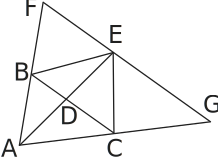
\includegraphics[width=0.26\textwidth]{%
gesamttex/edit_VIII,3/images/LH_35_10_07_009-010_d8_010r.pdf%
}}
\vspace{0.5em}
\centerline{%
\hspace{-95mm}%
\lbrack\textit{Fig.~7}\rbrack%
\label{LH_35_10_07_010r_Fig.7}%
}
% \newpage%
%\vspace{0.5em}
%
%
\vspace{-9.5em} %%%%%%%%% Diagramm 8
\centerline{%
\hspace{5mm}%
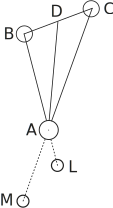
\includegraphics[width=0.20\textwidth]{%
gesamttex/edit_VIII,3/images/LH_35_10_07_009-010_d7_010r.pdf%
}}%
\vspace{0.25em}
\centerline{%
\hspace{5mm}%
\lbrack\textit{Fig.~8}\rbrack%
\label{LH_35_10_07_010r_Fig.8}%
}%
%\newpage%
%\vspace{1.0em}
%
\vspace{-13.2em} %%%%%%%%% Diagramm 9
\centerline{%
\hspace{100mm}%
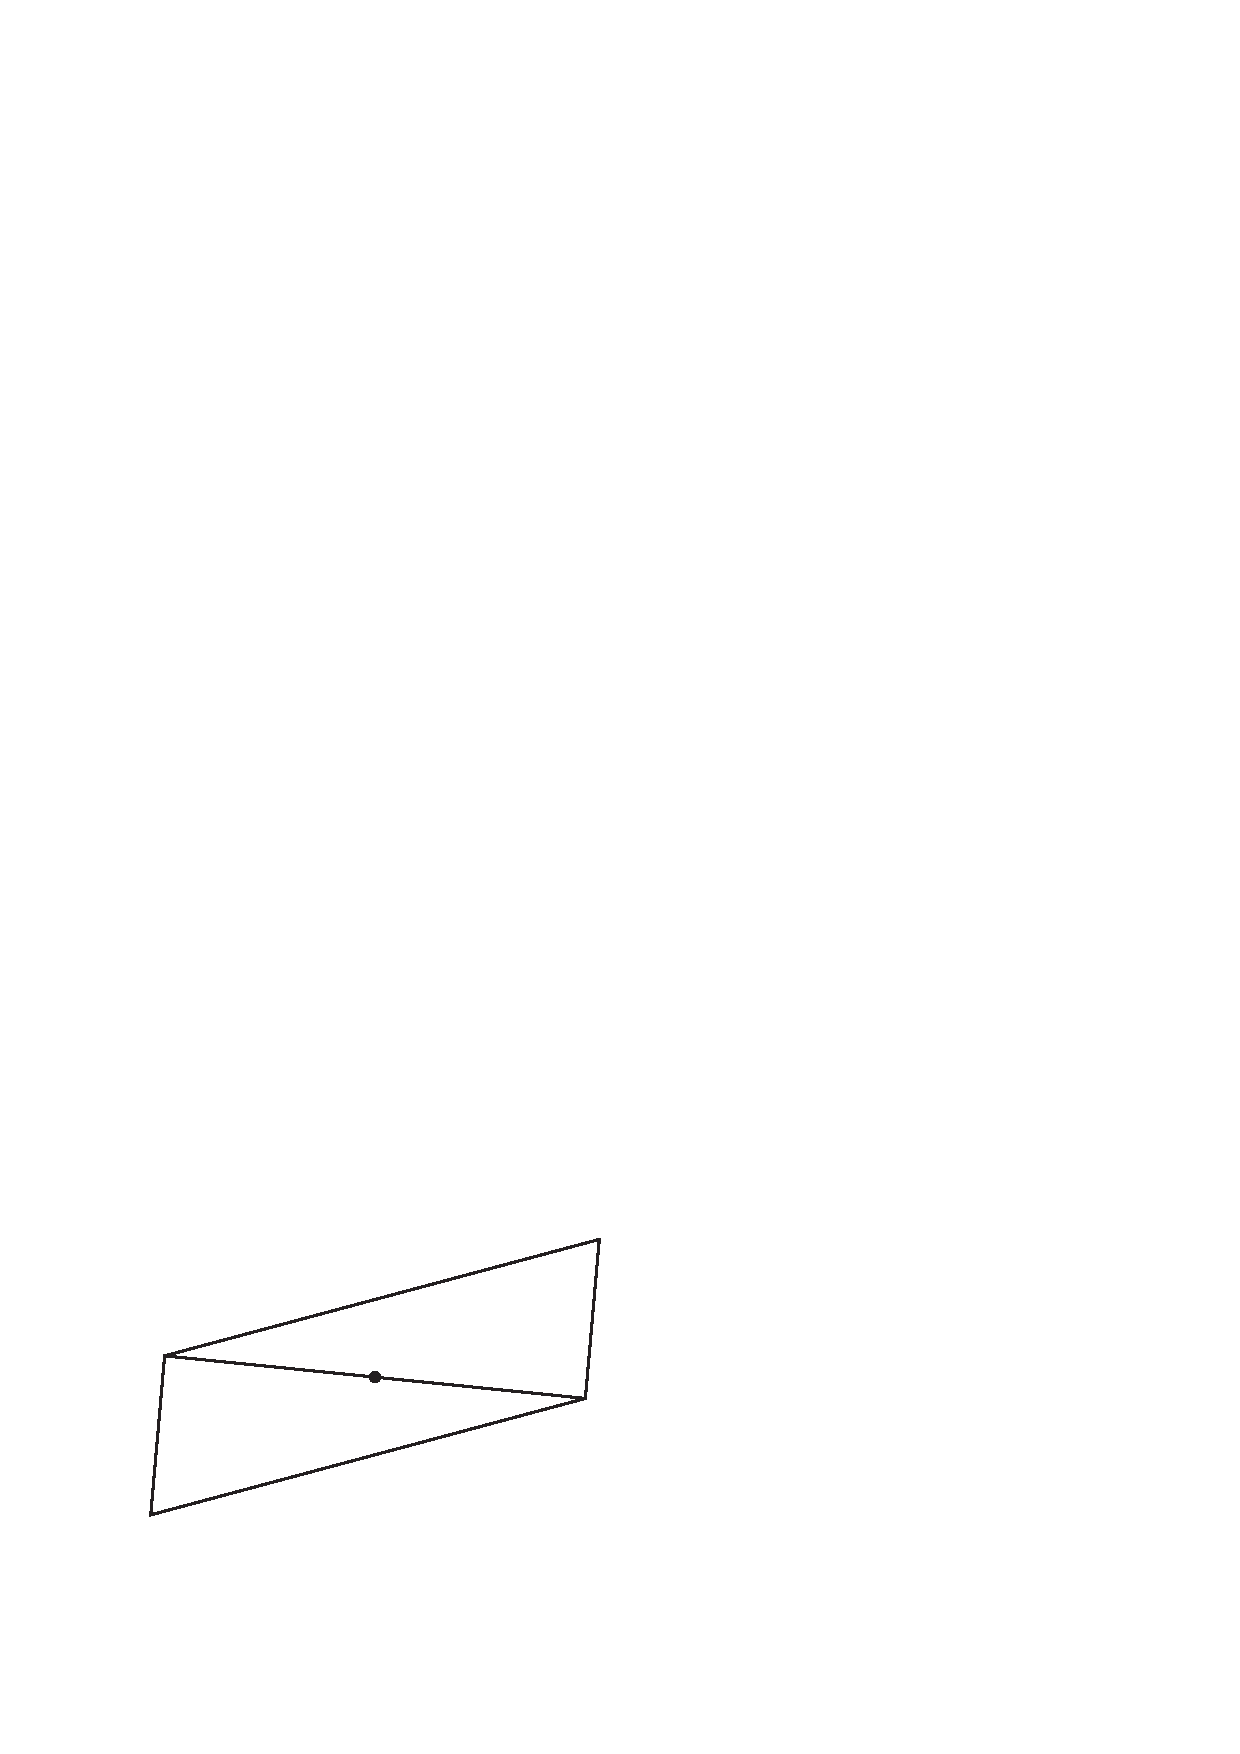
\includegraphics[width=0.2\textwidth]{%
gesamttex/edit_VIII,3/images/LH_35_10_07_009-010_d9_010r.pdf%
}}
\vspace{0.0em}
\centerline{%
\hspace{100mm}%
\lbrack\textit{Fig.~9}\rbrack%
\label{LH_35_10_07_010r_Fig.9}%
}
\newpage%
%\vspace{1.0em}
%
\pstart%
Nam corpus dimidiae levitatis%
\protect\index{Sachverzeichnis}{levitas specifica}
debet progredi duplo celerius,
ut eadem sit quantitas progressus,%
\protect\index{Sachverzeichnis}{quantitas progressus}
nempe in \textit{F} et in \textit{G}.
Verum difficultas est,%
\protect\index{Sachverzeichnis}{difficultas}
quod non videtur sumenda eadem quantitas progressus%
\protect\index{Sachverzeichnis}{quantitas progressus}
sed eadem quantitas potentiae.%
\protect\index{Sachverzeichnis}{quantitas potentiae}
Sed responderi potest,
eandem esse quantitatem progressus,%
\protect\index{Sachverzeichnis}{quantitas progressus}
sed non mutari ideo quantitatem potentiae,%
\protect\index{Sachverzeichnis}{quantitas potentiae}
quae pendet ex consideratione causae,%
\protect\index{Sachverzeichnis}{consideratio causae}
quae corpori \textit{A} duplices illos conatus%
\protect\index{Sachverzeichnis}{conatus duplex}%
\protect\index{Sachverzeichnis}{causa conatus duplicis}
impressit.
Ponamus scilicet corpora duo \textit{L} et \textit{M}
incurrere in corpus \textit{A},
ajo debere eandem esse quantitatem progressus%
\protect\index{Sachverzeichnis}{quantitas progressus}
in recta \textit{LB} et parallelis
ante et post concursum,%
\protect\index{Sachverzeichnis}{concursus plurium corporum}
et similiter 
%
\edtext{etiam eandem}{%
\lemma{etiam}\Bfootnote{%
\textit{(1)}~ante
\textit{(2)}~eandem%
~\textit{L}}}
%
esse debere quantitatem progressus%
\protect\index{Sachverzeichnis}{quantitas progressus}
in recta \textit{MC} et parallelis.
Praeterea eandem debere esse
\edlabel{35_10_07_009-010_1a}%
potentiam.%
\protect\index{Sachverzeichnis}{potentia corporum concurrentium}%
%
\edtext{}{%
{\xxref{35_10_07_009-010_1a}{35_10_07_009-010_1b}}%
{\lemma{potentiam\protect\index{Sachverzeichnis}{potentia}}\Bfootnote{%
\textit{(1)}~Omnium corporum quanti
\textit{(2)}~Quantitas
\textit{(a)}~progressus
\textit{(b)}~appropinquationis\protect\index{Sachverzeichnis}{appropinquatio} quotcunque corporum,
\textit{(aa)}~quae aliunde non
\textit{(bb)}~aliunde
\textit{(aaa)}~non
\textit{(bbb)}~nihil
\textit{(3)}~quantitas
\textit{(4)}~accessus aut recessus quotcunque corporum
\textit{(5)}~Quantitas appropinquationis\protect\index{Sachverzeichnis}{quantitas appropinquationis}
\textit{(6)}~Celeritas
\textit{(7)}~Quantitas appropinquationis
\textbar~vel elongationis \textit{erg.}~%
\textbar\ quotcunque corporum ad idem
\textit{(8)}~Quantitas progressus
\textit{(9)}~Quotcunque corporum
\textbar~nihil ab aliis, extra ipsa
\textbar~ivicem \textit{ändert Hrsg.}~%
\textbar~, patientium quantitas progressus \textit{erg.}~%
\textbar\ respectu distantiae % a dato quovis puncto, semper 
\lbrack...\rbrack\ est aequalis,
\textit{(a)}~si scilicet corpora haec nihil ab aliis extraneis extra ipsa pati intelligantur.
\textit{(b)}~seu
\textit{(aa)}~eadem est
\textit{(bb)}~puncto illo % eodem assumto, eadem semper est quantitas centripeta 
\lbrack...\rbrack\ vel centrifuga.%
~\textit{L}}}}%
%
\pend%
%
\pstart%
%
Quotcunque corporum nihil ab aliis,
extra ipsa
\lbrack invicem\rbrack,
patientium quantitas progressus%
\protect\index{Sachverzeichnis}{quantitas progressus}
respectu distantiae a dato % ,
quovis puncto % ,
semper est aequalis
seu\lbrack,\rbrack\
puncto illo eodem assumto,
eadem semper est
\edlabel{LH_35_10_07_0010r_centripetafuga-1}%
quantitas centripeta%
\protect\index{Sachverzeichnis}{quantitas centripeta}
vel centrifuga.%
\protect\index{Sachverzeichnis}{quantitas centrifuga}%
\edlabel{LH_35_10_07_0010r_centripetafuga-2}%
\edlabel{35_10_07_009-010_1b}%
%
\pend%
%
%
%
% % % %    Ende des Textes auf Bl. 10r.
\count\Afootins=1200%
\count\Bfootins=1200%
\count\Cfootins=1200